\section{Reinforcement learning algorithm}
\label{sec:rl}

\textbf{pm: under construction do not change}

Given a stochastic policy $\pi$, which for a given state assigns probability distribution over possible actions, we define the value function $V_\pi(s) := \mathbb{E}_{\pi}\left(\sum_{t=0}^{+\infty}\gamma^t r_{t+1}|s=s_0 \right)$. We define $\eta(\pi)$ to be the value function, when the initial state is sampled according to $\rho_0$. The goal of reinforcement learning is to find a policy which maximizes $\eta$.

In our experiments the reinforcement learning part of the loop in Figure \ref{figure_basic_loop} (Algorithm \ref{basic_loop}, line 6) is performed with the Proximal Policy Optimization algorithm (PPO, \cite{ppo}). PPO is a general purpose model-free reinforcement learning algorithm. This kind of algorithm can be considered as a black-box in this project. The black-box works for a prescribed number of epochs. In a single epoch it gathers new episodes and using experience from the episodes it improves the policy. % The procedure is motivated by the DAgger algorithm \cite{dagger} and presented below in Algorithm \ref{basic_loop}.

\paragraph{Training of a reinforcement learning agent}
% TODO: details about PPO, update figure below.
% latex source https://www.overleaf.com/16266511yhyscgmyhztg
% \begin{figure}[H]
% \centering
% 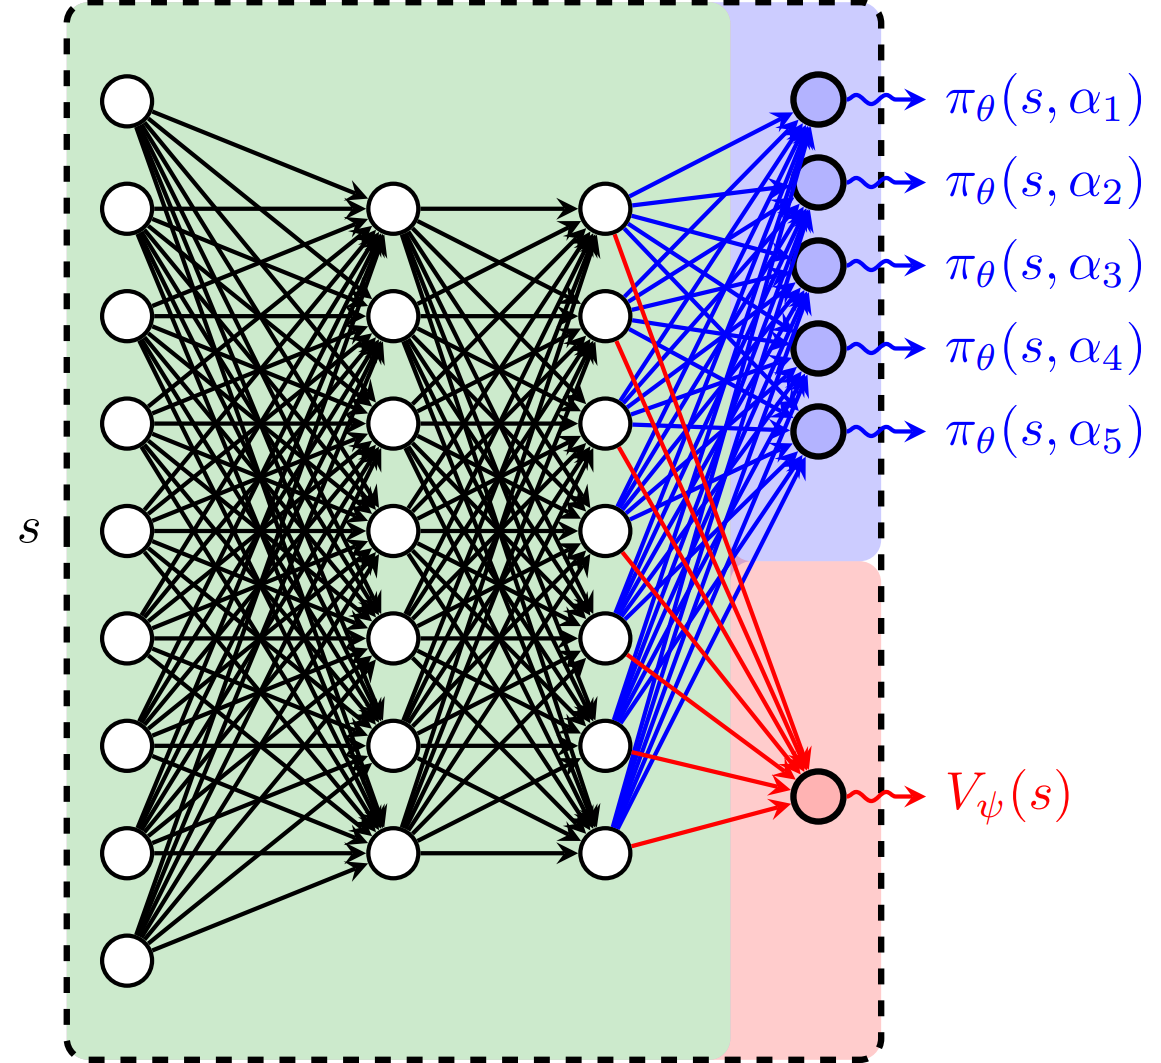
\includegraphics[width=4in]{figures/network_ppo.png}
%  \end{figure}